\section*{Problema 4}

\textbf{Considera los datos \file{oef2.data}. Se trata de los promedios mensuales de la temperatura (en Celsius) en 35 estaciones canadienses de monitoreo. El interés es comparar las estaciones entre sí en base de sus curvas de temperatura. Considerando las 12 mediciones por estación como un vector X, aplica un análisis de componentes principales. Como X representa (un muestreo de) una curva, este tipo de datos se llama datos funcionales.Interpreta y dibuja (como curva) los primeros dos componentes, p\textsubscript{1}, p\textsubscript{2}, es decir grafica \{(i, p\textsubscript{1i})\} y \{(i, p\textsubscript{2i})\}. Agrupa e interpreta las estacionesen el biplot (ten en mente un mapa de Canada).}

En la figura \ref{fig:components} se muestra las gráficas lineales de los valores de cada componente. Se observa que el comportamiento es semejante en las dos componentes. La primer componente conserva una menor variación en sus valores a comparación de la segunda componente.

\begin{figure}[H]
    \centering
    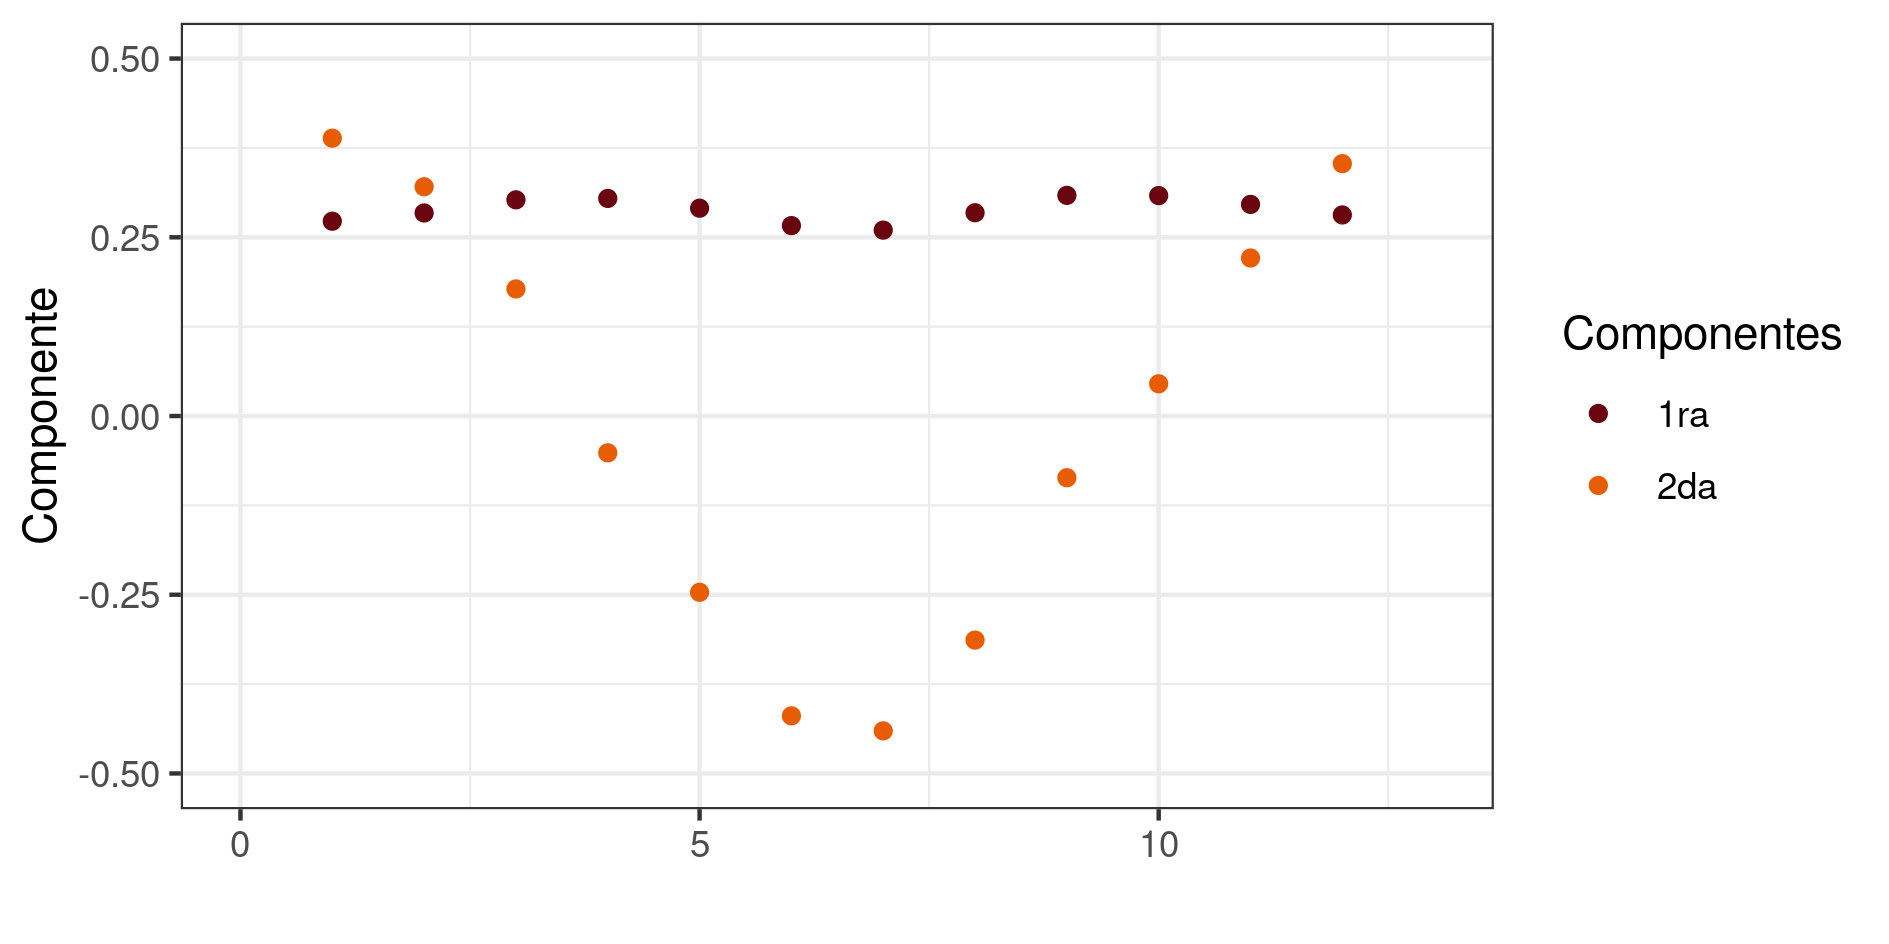
\includegraphics[width=13cm]{Graphics/components.png}
    \caption{Valores de la primer y segunda componente obtenida con PCA.}
    \label{fig:components}
\end{figure}

\begin{figure}[H]
    \centering
    \begin{subfigure}{8cm}
        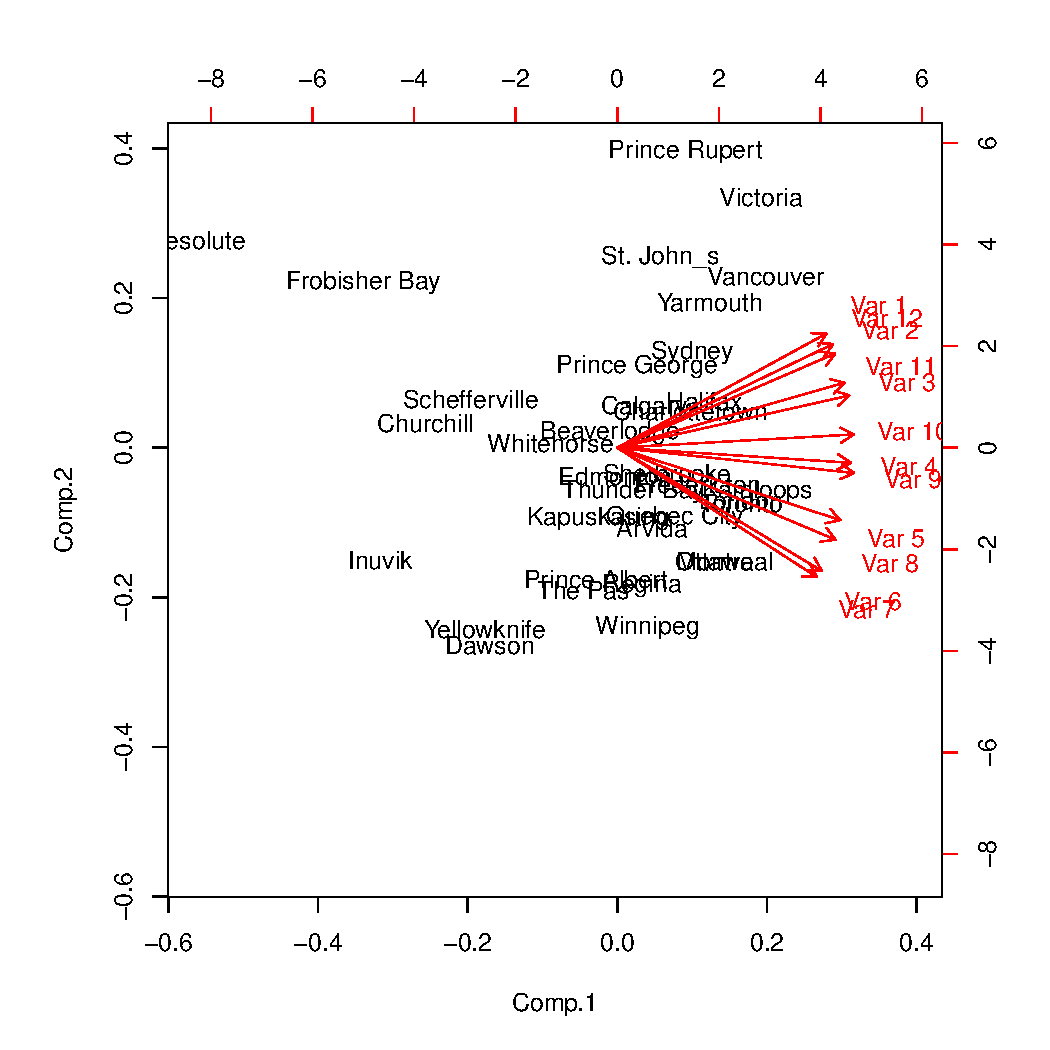
\includegraphics[width=8cm]{Graphics/biplot.pdf}
        \caption{Biplot de la primer y segunda componente obtenido de los datos del archivo \file{oef2.data}.}
        \label{fig:biplot}
    \end{subfigure}
    \hspace{0.5cm}
    \begin{subfigure}{8cm}
        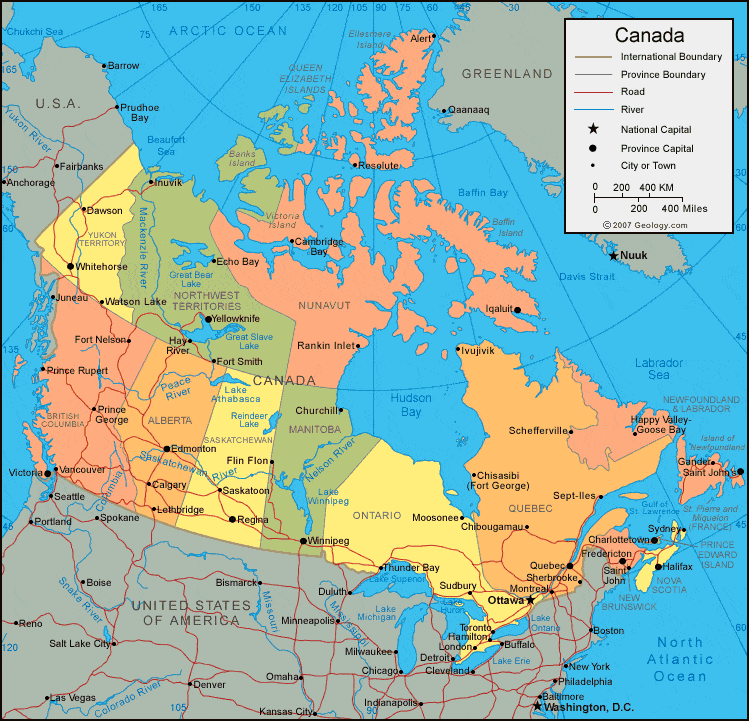
\includegraphics[width=8cm]{Graphics/canada-map.png}
        \caption{Mapa de Canada. Obtenido de \href{https://geology.com/world/canada-satellite-image.shtml}{Geology.com}}
        \label{fig:canada_map}
    \end{subfigure}
    \caption{}
\end{figure}

En la figura \ref{fig:biplot} se muestra la gráfica de biplots obtenida al aplicar PCA a los datos del archivo \file{oef2.data}. Se observa como la distribución de valores se concentra para las estaciones que tienen una latitud semejante (figura \ref{fig:canada_map}). En cambio para la estación ubicada en Resolute se encuentra lejana de las demás. Esto puede dar la interpretación que mientras más se encuentren en la izquierda de la gráfica las estaciones reportaran una temperatura menor. En caso contrario, estas reportaran una temperatura mayor.
